\chapter{after effects} 
\label{sec:patterns}
\rhead[]{\leftmark}
\lstset{style=6502Style}
\lstset{ 
   aboveskip=5pt,
   belowskip=0pt,
}
After Psychedelia, Jeff Minter\index{Minter} spent the rest of his working life make 'light synthesizers' of one sort or another. We will cover the very next incarnation of the
Psychedelia concept in our companion volume 'Colourspace Complex', an exploration of the 1985 title 'Colourspace' written just a few months after the C64\index{C64} original
which took advantage of the superior graphical capabilities and colour palette of the Atari 800. 

But Minter\index{Minter} himself didn't stop with the Atari 800. He went on to develop the light
synthesiser concept on nearly every generation of video game console released
over the next thirty years. Some of these efforts were doomed by the failure of
the platform they were written for, such as the 'Virtual Light Machine\index{Virtual Light Machine}' on the
ill-fated Atari Jaguar and the 'VLM 1' for the now rapidly defunct Nuon DVD platform developed by
VM Labs. This chequered history culminated in something of a small triumph, when his PC-generation version of the Virtual Light Machine\index{Virtual Light Machine} engine, known as 'Neon',
was incorporated into the XBOX 360 when it was released in 2005. For the first time in his career, Minter\index{Minter}'s light synthesizer went mainstream and was put in the
hands of millions of customers.

For us though, we will end in 1985, with Minter\index{Minter}'s final iteration of his light machine on 8-bit hardware: a psychedelic sub-game in his 1985 title 'Batalyx\index{Batalyx}'. Here
we find the idea reduced again to its kernel, back to a version of its beginnings in PC Computer Weekly magazine as a short lump of code that can fit on a few pages.
Like the listing we acquainted ourselves at the start of this book, the version of Psychedelia in 'Batalyx\index{Batalyx}' supports only a single lightform (or pattern) and only
minimal configuration. Minter\index{Minter}'s motivation was simple:

\subfile{after_effects/batalyx_listing.tex}

\begin{figure}[H]
    \centering
    \begin{adjustbox}{width=11cm,center}
      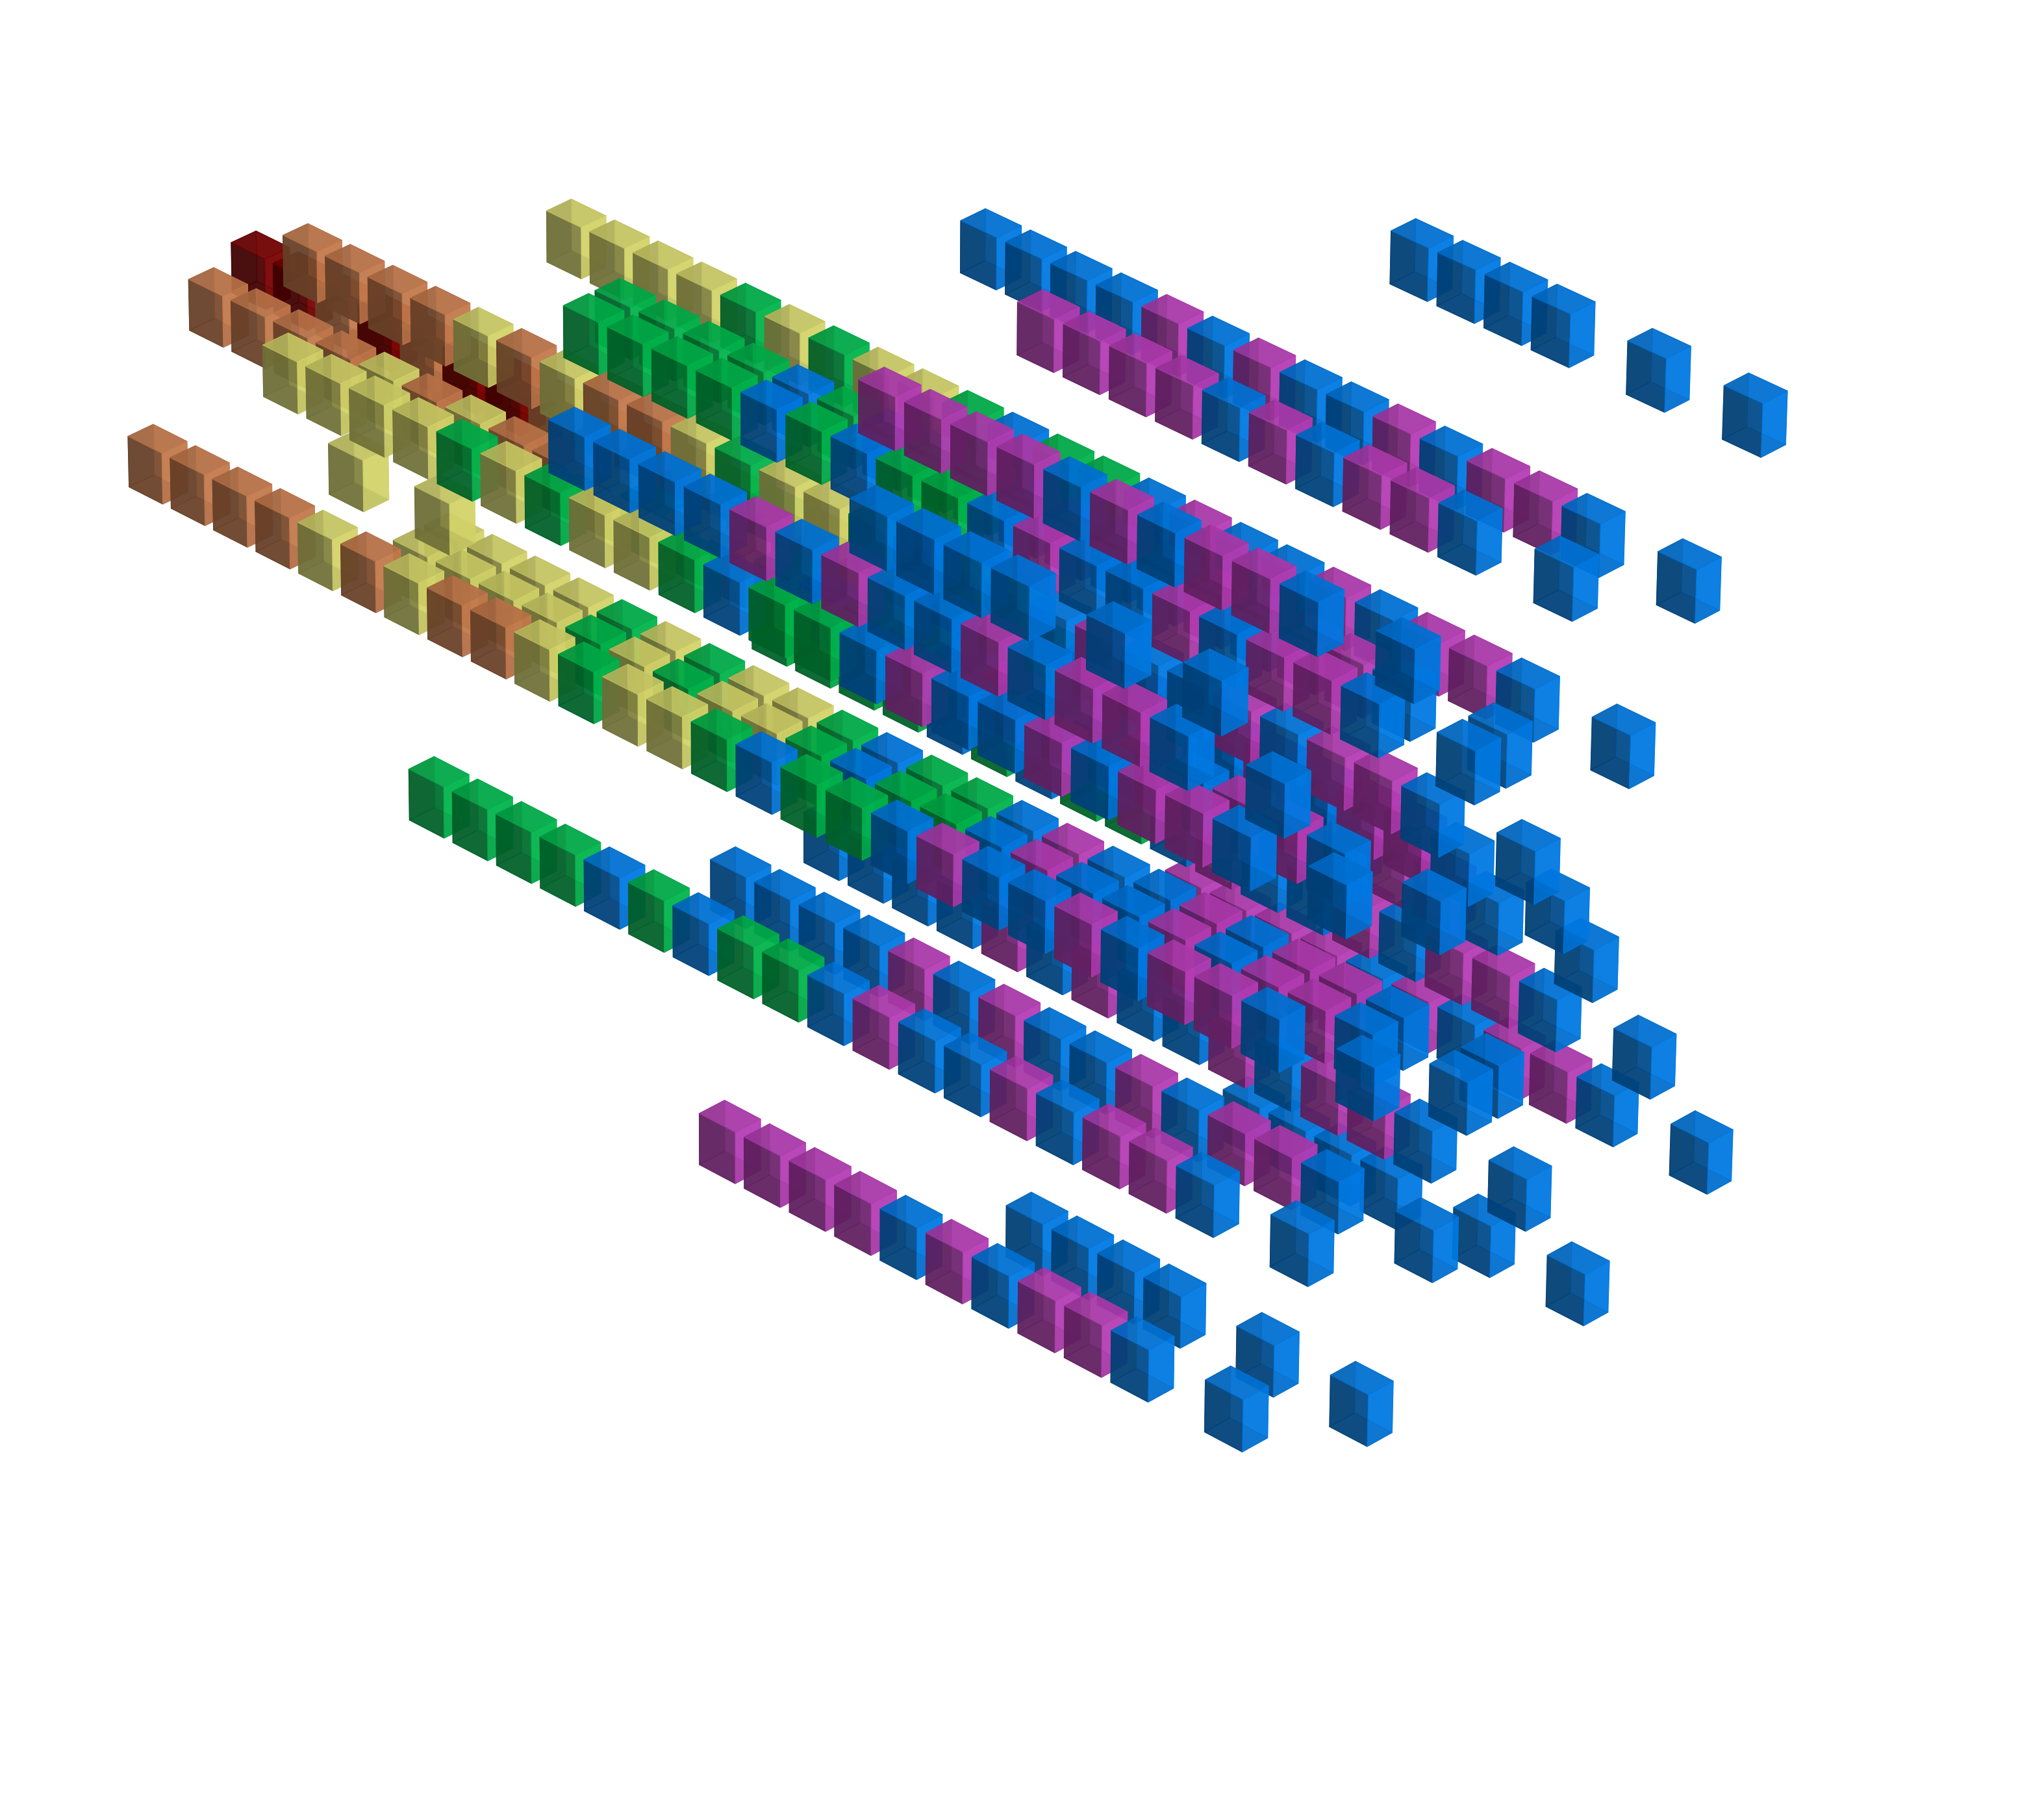
\includegraphics[width=11cm]{src/batalyx_patterns/pattern0-45.png}%
    \end{adjustbox}
    \begin{adjustbox}{width=11cm,margin=0cm -2cm}
      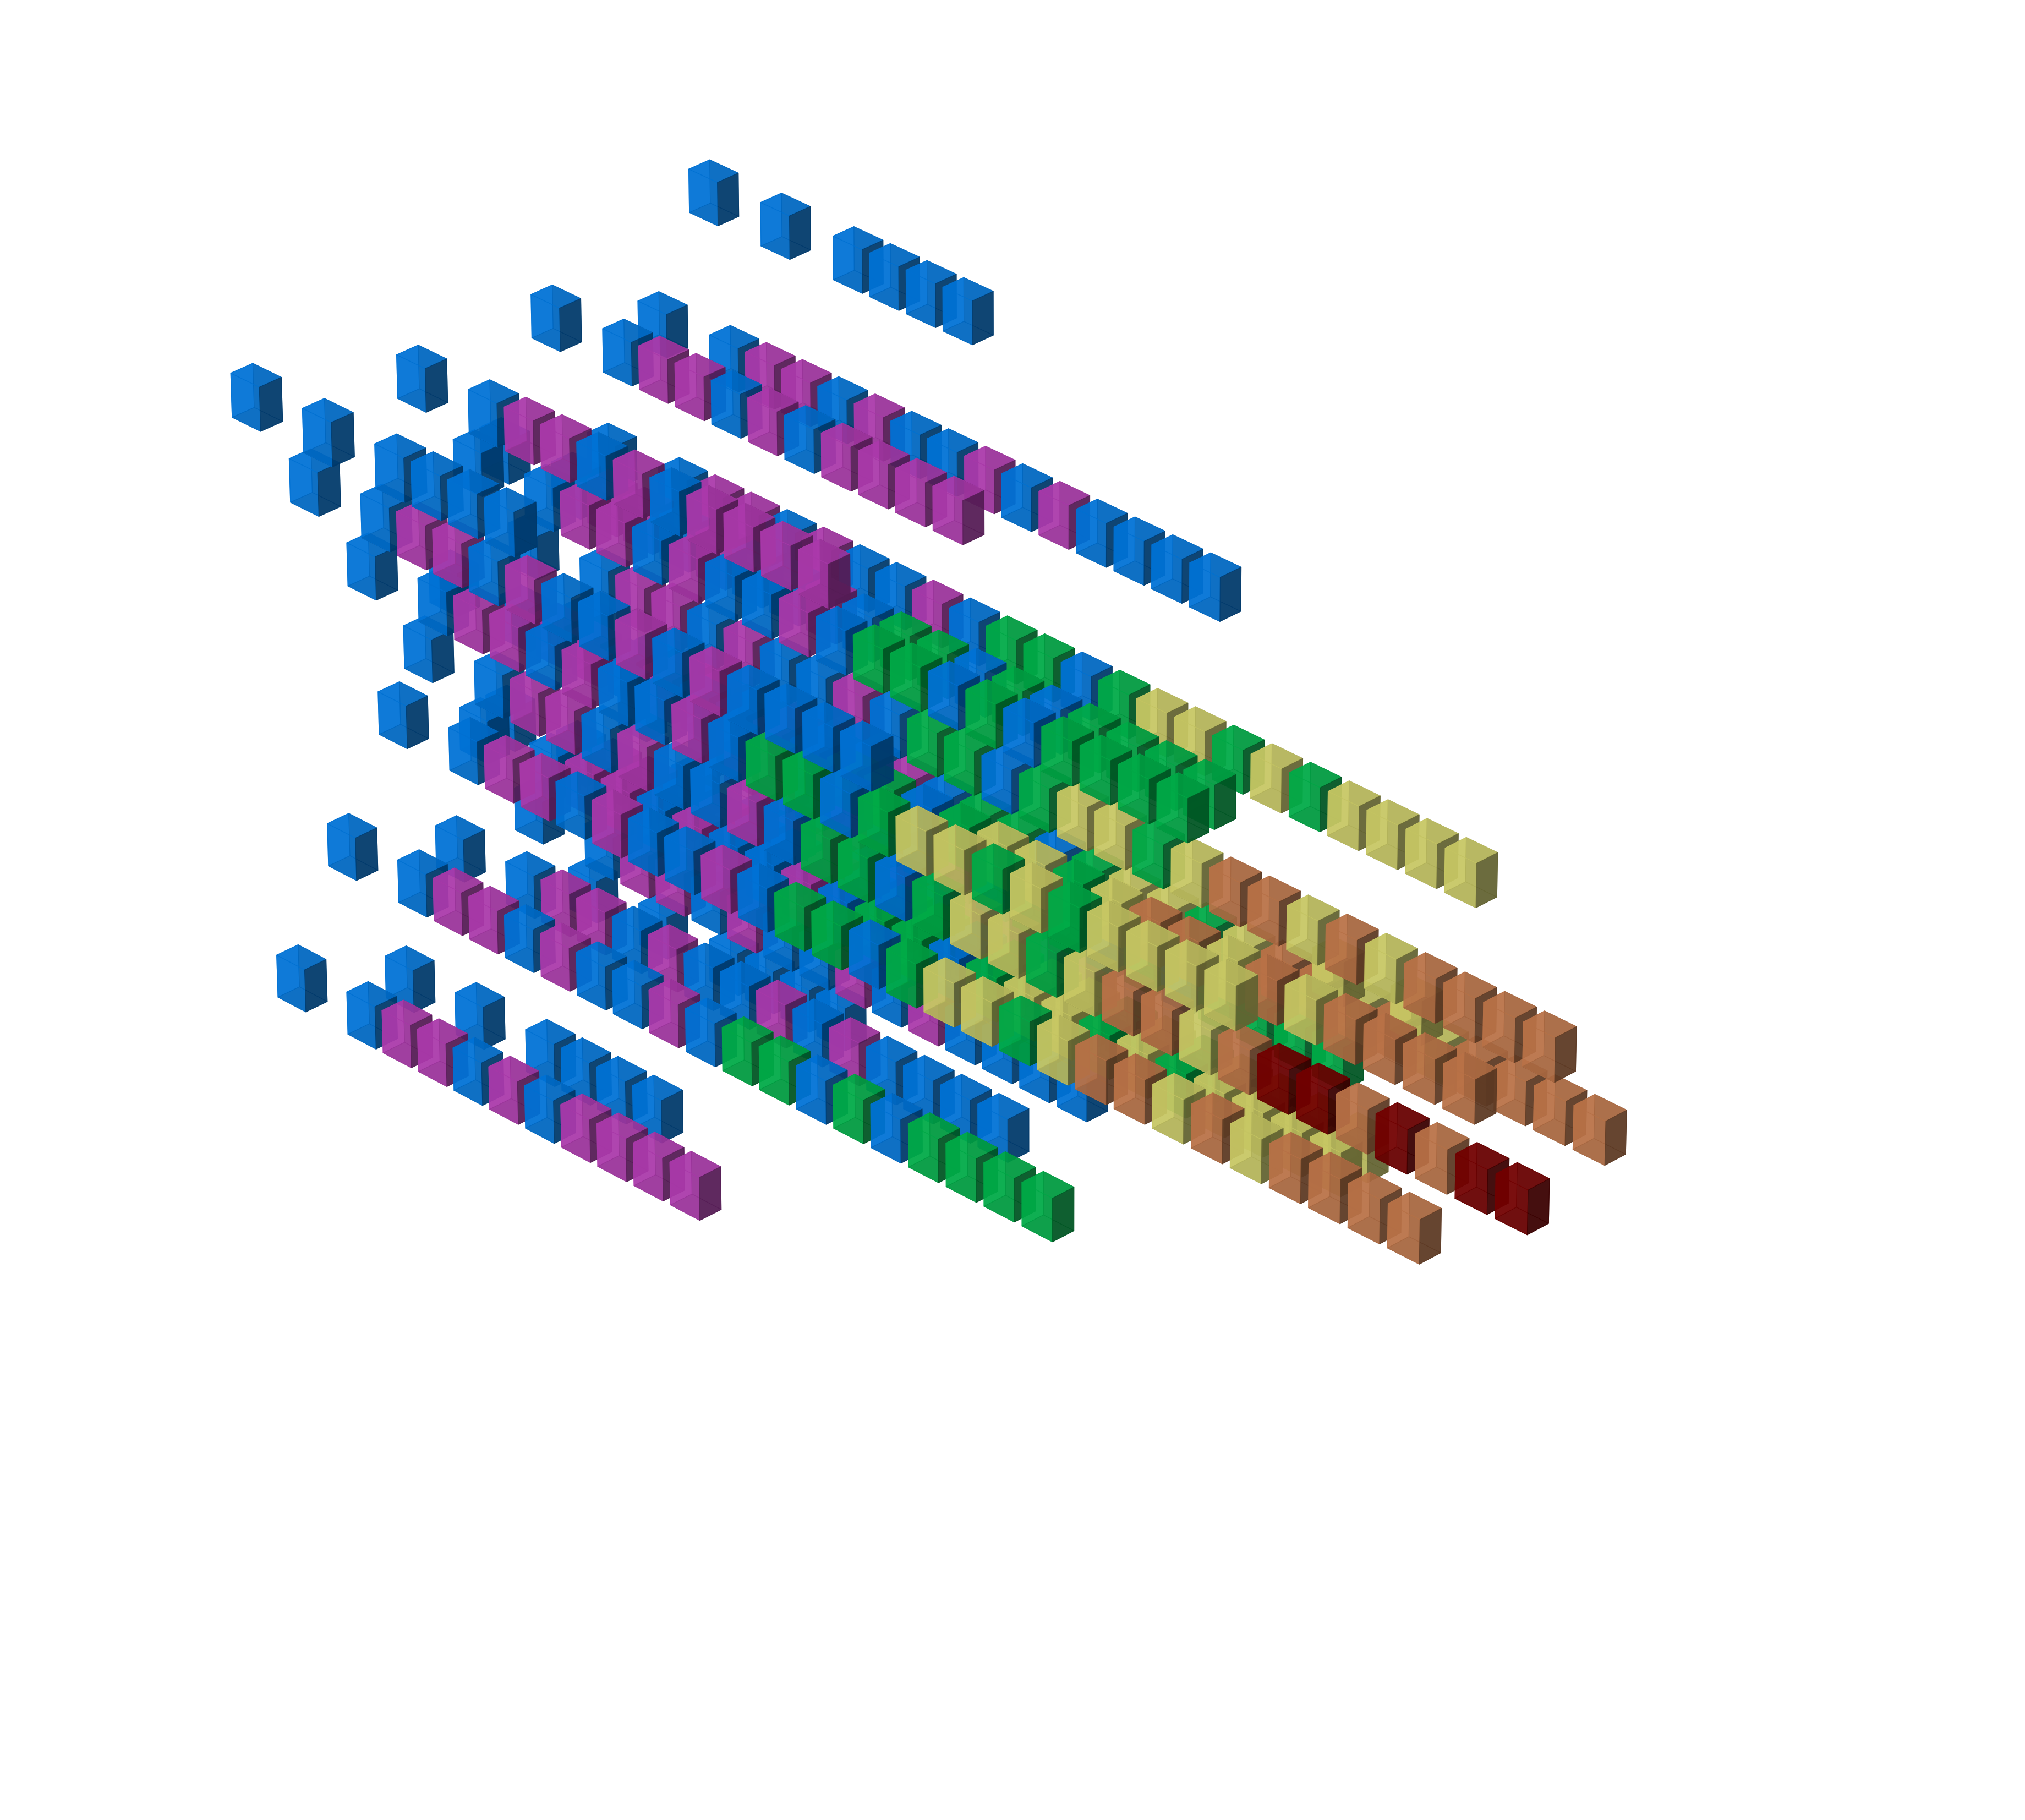
\includegraphics[width=11cm]{src/batalyx_patterns/pattern0-225.png}%
    \end{adjustbox}
\caption{Evolution of the 'Batalyx\index{Batalyx}' pattern.}
\end{figure}

\rhead[]{Star One}
\begin{lstlisting}[caption=Source code for the Batalyx\index{Batalyx} pattern..,escapechar=\%]
patternXPosArray             
        .BYTE $FF,$01,$55    ; 6              
        .BYTE $FE,$02,$55    ;            5   
        .BYTE $FD,$03,$55    ;   4            
        .BYTE $FC,$04,$55    ;          3     
        .BYTE $FB,$05,$55    ;     2          
        .BYTE $FA,$06,$55    ;        1       
        .BYTE $55,$55        ;                
patternYPosArray             ;      1         
        .BYTE $01,$FF,$55    ;         2      
        .BYTE $FE,$02,$55    ;    3           
        .BYTE $03,$FD,$55    ;           4    
        .BYTE $FC,$04,$55    ;  5             
        .BYTE $05,$FB,$55    ;             6 
        .BYTE $FA,$06,$55
        .BYTE $55,$55
\end{lstlisting}

\subfile{batalyx_patterns/tables/pattern0.tex}

\clearpage
\textbf{Lines 41-55. \icode{\textbf{LaunchPsychedelia\index{LaunchPsychedelia}}}} 
\begin{lstlisting}[escapechar=\%]
;--------------------------------------------------------
; LaunchPsychedelia%\index{LaunchPsychedelia}%
;--------------------------------------------------------
LaunchPsychedelia%\index{LaunchPsychedelia}%
        SEI 
        JSR InitializePsychedelia
        JSR SetUpBackgroundPainting
        JSR InitializeColorIndexArray
        JSR InitializeStatusDisplayText
        JSR UpdateCurrentSettingsDisplay
        CLI 
PsychedeliaLoop   
        JSR MaybeUpdateFromBuffersAndPaint
        JSR CheckKeyboardInput%\index{CheckKeyboardInput}%
        JMP PsychedeliaLoop
\end{lstlisting}
\textbf{Lines 805-841. \icode{\textbf{MaybeUpdateFromBuffersAndPaint}}} 
\begin{lstlisting}[basicstyle=\ttfamily\scriptsize, caption=The routine responsible for painting patterns.,escapechar=\%]
MaybeUpdateFromBuffersAndPaint   
        LDX currentIndexToPixelBuffers%\index{currentIndexToPixelBuffers}%
        LDA currentColorIndexArray%\index{currentColorIndexArray}%,X
        AND #$08
        BNE BufferUpdateComplete

        DEC smoothingDelayArray,X%\index{smoothingDelayArray,X}%
        BNE BufferUpdateComplete

        LDA initialSmoothingDelayArray%\index{initialSmoothingDelayArray}%,X
        STA smoothingDelayArray,X%\index{smoothingDelayArray,X}%

        LDA pixelXPositionArray%\index{pixelXPositionArray}%,X
        STA currentPixelXPosition
        LDA pixelYPositionArray%\index{pixelYPositionArray}%,X
        STA currentPixelYPosition

        LDA currentColorIndexArray%\index{currentColorIndexArray}%,X
        STA currentColorIndex

        TAY 
        LDA symmetrySettingForStep,X
        STA currentSymmetrySettingForStep%\index{currentSymmetrySettingForStep}%

        LDA presetColorValuesArray%\index{presetColorValuesArray}%,Y
        STA currentColor

        INC currentColorIndexArray%\index{currentColorIndexArray}%,X
        JSR PaintStructureAtCurrentPosition%\index{PaintStructureAtCurrentPosition}%

BufferUpdateComplete   
        INC currentIndexToPixelBuffers%\index{currentIndexToPixelBuffers}%

        LDA currentIndexToPixelBuffers%\index{currentIndexToPixelBuffers}%
        AND #$3F
        STA currentIndexToPixelBuffers%\index{currentIndexToPixelBuffers}%
        RTS 
\end{lstlisting}
\clearpage

\rhead[]{\icode{LaunchPsychedelia\index{LaunchPsychedelia}}}
\textbf{Lines 41-55. \icode{\textbf{LaunchPsychedelia\index{LaunchPsychedelia}}}:} A nice compact launch routine compared to what we're used to. As an added
bonus it also contains the game's main loop in \icode{PsychedeliaLoop}! The first thing to note here is that, unlike all the previous
versions we've looked at, this main loop is also checking keyboard input - something previously managed by the interrupt handler. The
interrupt handler, as well as animating the background, still looks after joystick input but the reduced set of keyboard commands and
the increased load on the interrupt handler, means that we can fit the keyboard check in here instead.

Of course \icode{PsychedeliaLoop}'s main purpose in life is to repeatedly call \icode{MaybeUpdate\-FromBuffersAndPaint}.

\bigskip
\bigskip
\bigskip
\bigskip
\bigskip

\textbf{Lines 805-841. \icode{\textbf{MaybeUpdateFromBuffersAndPaint}}:} The business end of the main loop which co-ordinates
all pattern painting. The logic used to determine whether a paint looks superficially similar to Psychedelia, but there is
a subtle, yet ultimately critical, difference. Whereas Psychedelia managed the values 
in \icode{currentColorIndexArray\index{currentColorIndexArray}}by decrementing them and continuing to paint the pixel represented by that
position until it was decremented past zero, here we manage \icode{currentColorIndexArray\index{currentColorIndexArray}} by incrementing
it and ceasing painting once the value reaches \icode{\$08}, i.e. when there are no more colors to reference.


\clearpage
Below we see the very different execution profiles of the commercial edition of Psychedelia on the left and 
the 'Batalyx\index{Batalyx}' edition we are examining here. Rather than occuring in clusters, the painiting in this version
is much more evenly spread over time.
\vfill
\begin{figure}[H]                                                          
  \centering                                                             
  \begin{adjustbox}{width=13cm,center}                                   
  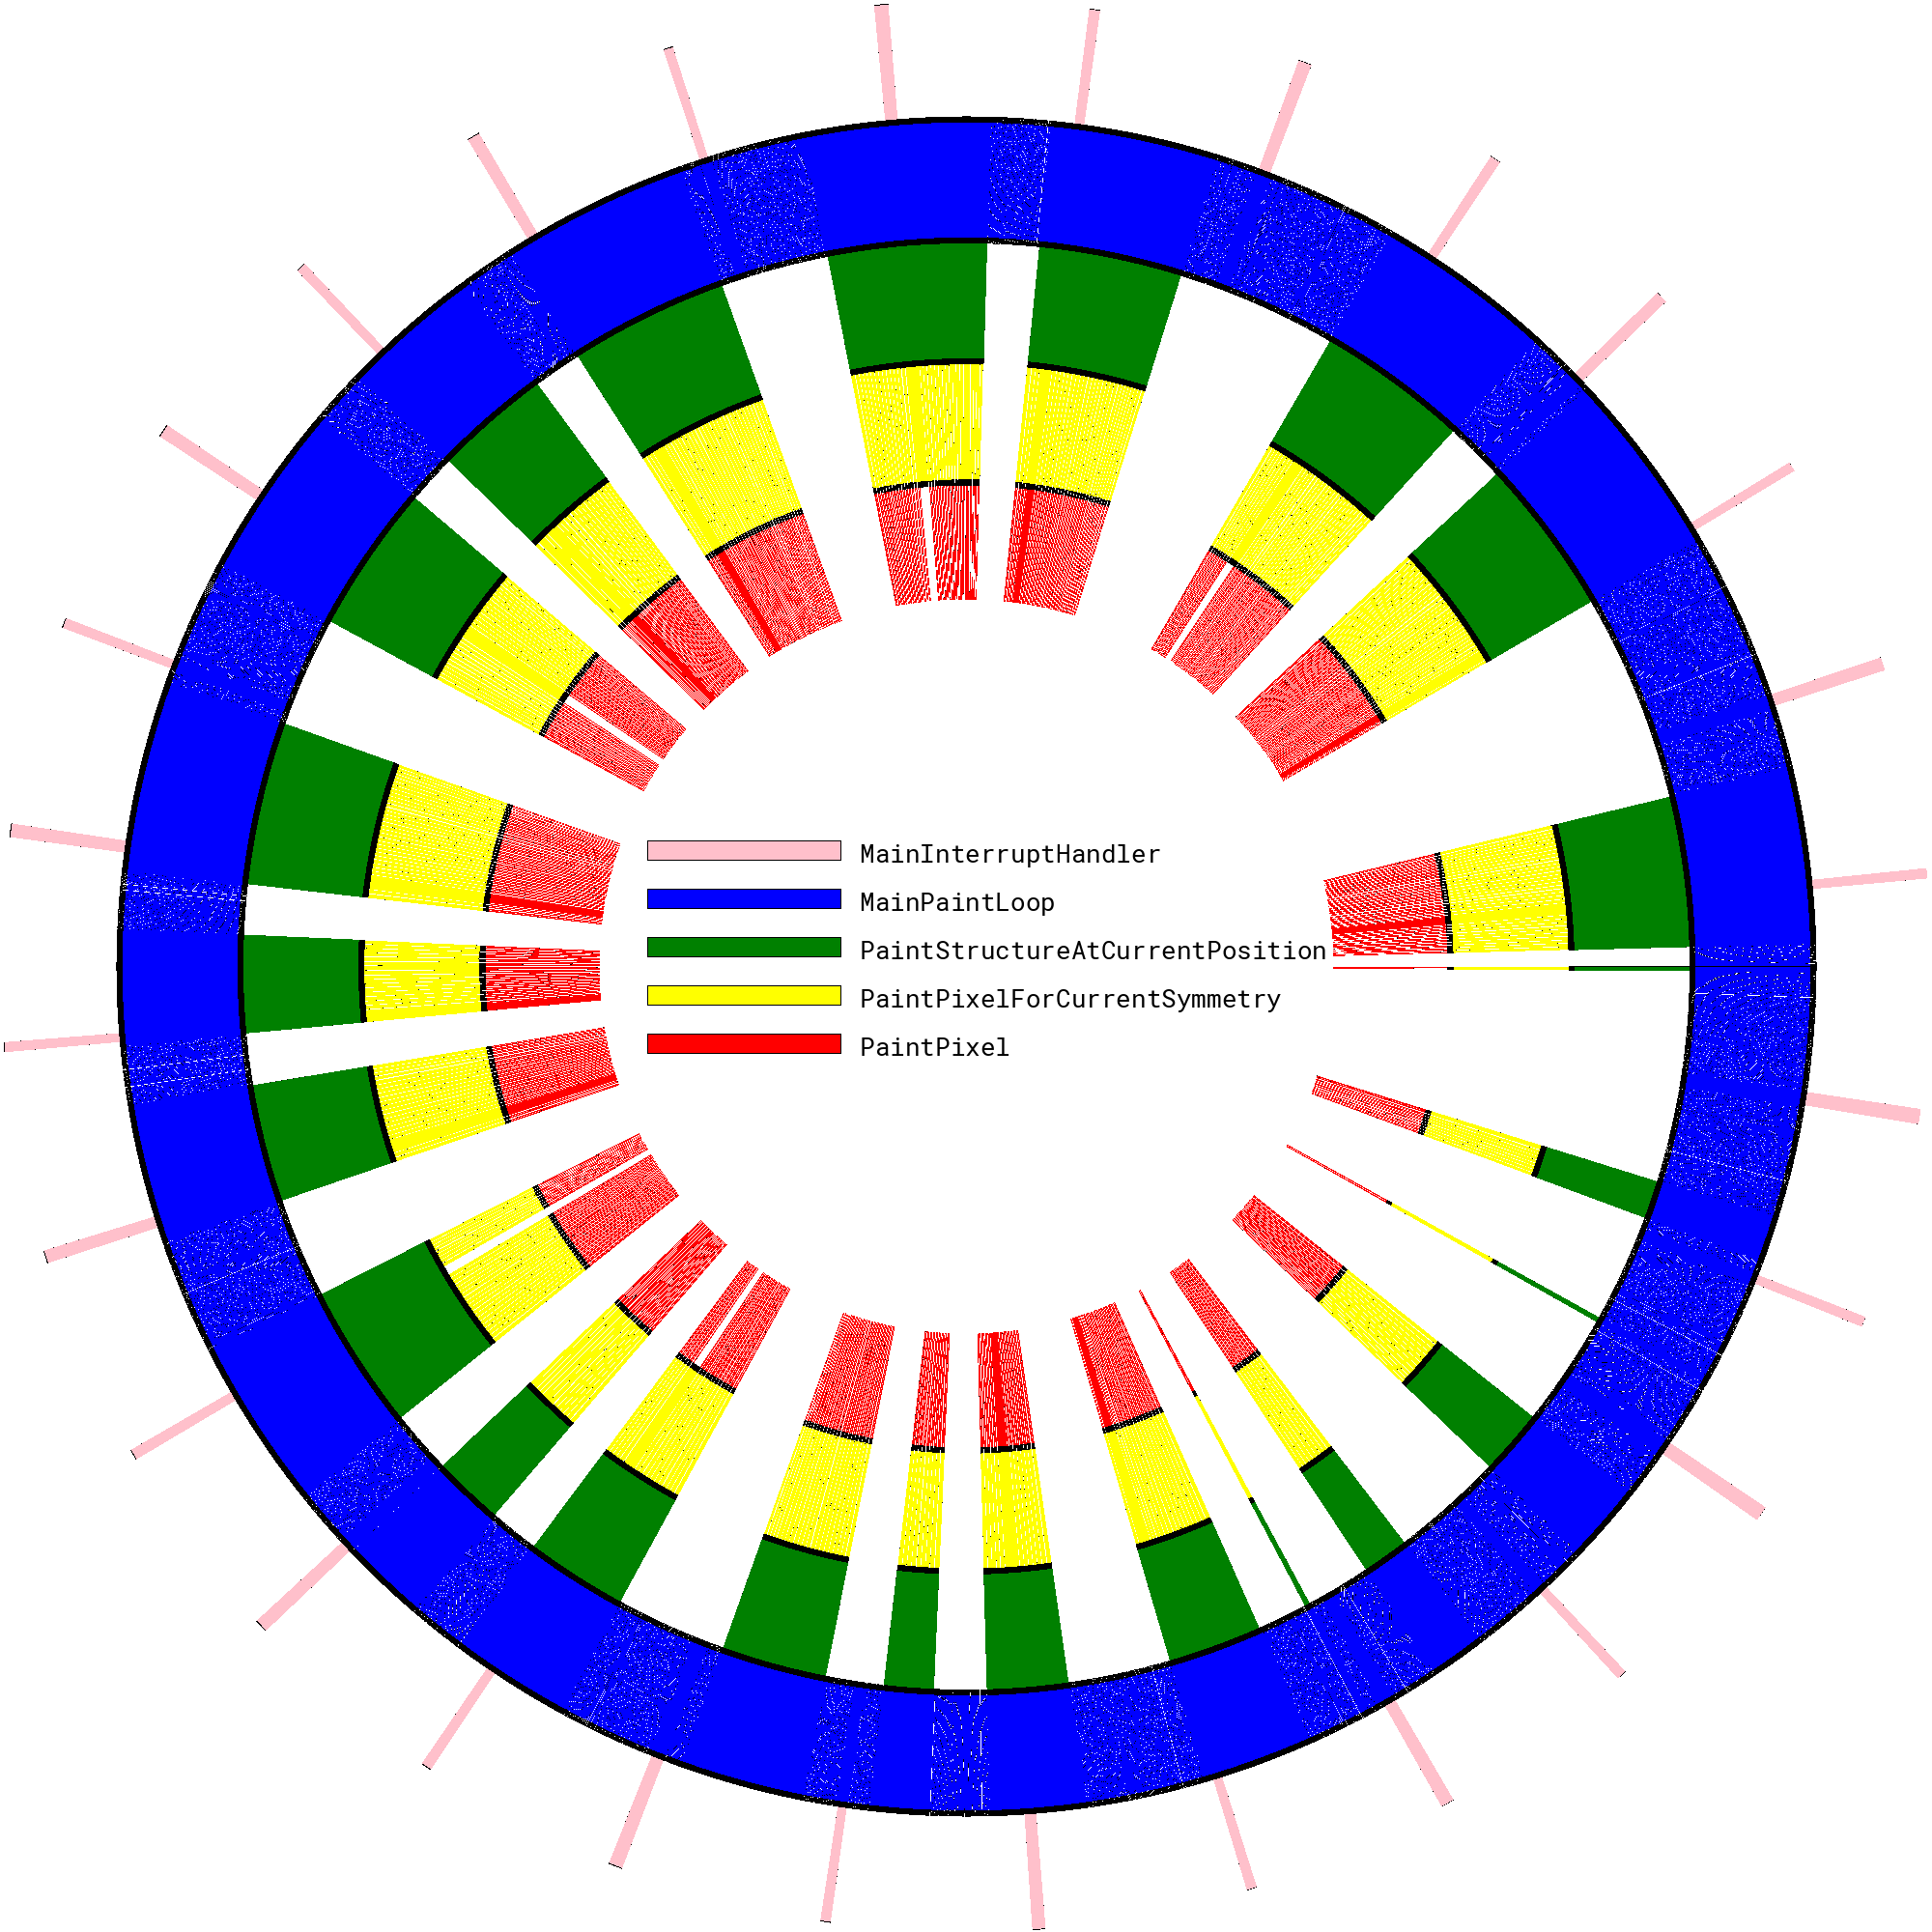
\includegraphics[width=13cm]{src/listing_commentary/execution_cycle.png}%           
  \end{adjustbox}                                                        
\caption{The execution map of a full pattern evolution in the original edition of Psychedelia.}                                           
\end{figure}                                                               
\clearpage
As we shall see, there is something new in the logic in
\icode{PaintStructureAtCurrentPosition\index{PaintStructureAtCurrentPosition}} that accounts for this change in behaviour.
\vfill
\begin{figure}[H]                                                          
  \centering                                                             
  \begin{adjustbox}{width=13cm,center}                                   
  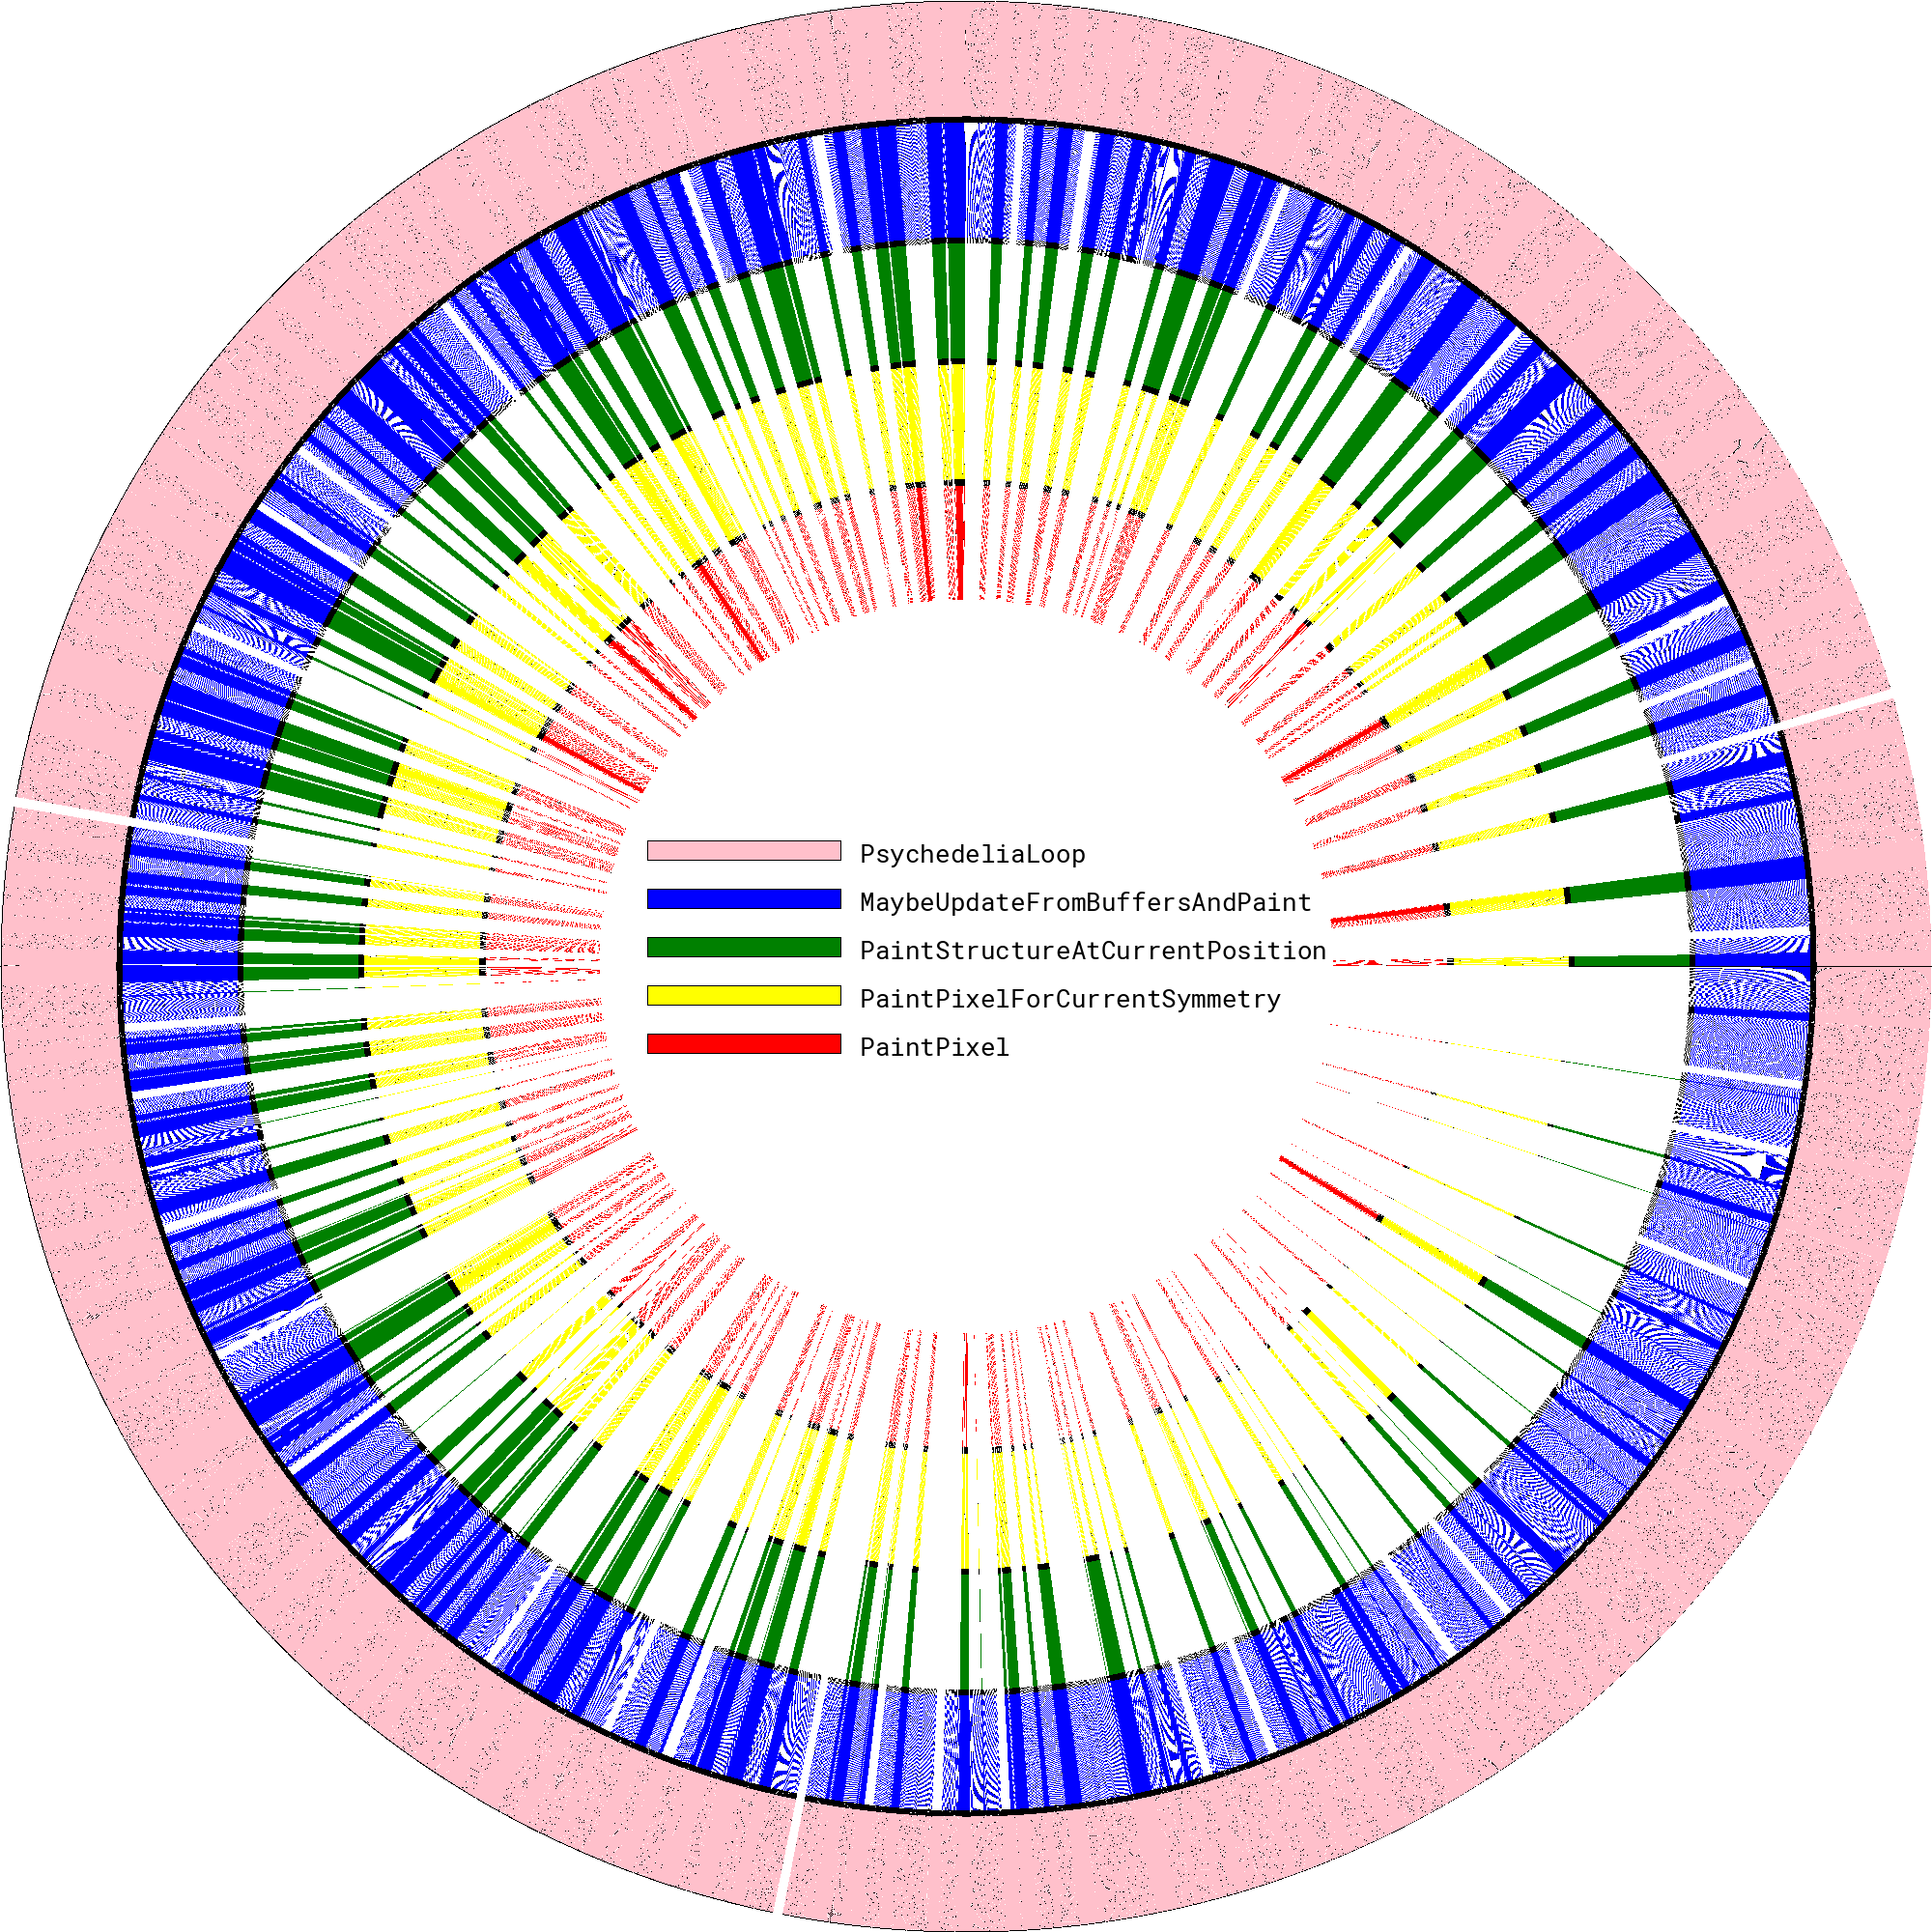
\includegraphics[width=13cm]{src/after_effects/execution_cycle.png}%           
  \end{adjustbox}                                                        
\caption{The execution map of a full pattern evolution in the Batalyx\index{Batalyx} edition of Psychedelia.}                                           
\end{figure}                                                               

\clearpage
\textbf{Lines 635-677. \icode{\textbf{PaintStructureAtCurrentPosition\index{PaintStructureAtCurrentPosition}}}} 
\begin{lstlisting}[caption = All the pattern data structures in Psychedelia organized into a set of arrays.,escapechar=\%]
;--------------------------------------------------------
; PaintStructureAtCurrentPosition%\index{PaintStructureAtCurrentPosition}%
;--------------------------------------------------------
PaintStructureAtCurrentPosition%\index{PaintStructureAtCurrentPosition}%   
        LDA #$00
        STA currentPatternIndex
        STA currentLineInPattern

        LDA currentPixelXPosition
        STA initialPixelXPosition
        LDA currentPixelYPosition
        STA initialPixelYPosition

        JSR PaintPixelForCurrentSymmetry%\index{PaintPixelForCurrentSymmetry}%

        LDA currentColorIndex
        BNE PixelPaintLoop%\index{PixelPaintLoop}%
        RTS 

PixelPaintLoop%\index{PixelPaintLoop}%   
        LDX currentPatternIndex
        LDA patternXPosArray,X
        CMP #$55
        BEQ MoveToNextLineInPattern

        CLC 
        ADC currentPixelXPosition
        STA initialPixelXPosition

        LDA patternYPosArray,X
        CLC 
        ADC currentPixelYPosition
        STA initialPixelYPosition

        JSR PaintPixelForCurrentSymmetry%\index{PaintPixelForCurrentSymmetry}%

        INC currentPatternIndex
        JMP PixelPaintLoop%\index{PixelPaintLoop}%

MoveToNextLineInPattern   
        INC currentPatternIndex
        INC currentLineInPattern
        LDA currentLineInPattern
        CMP currentColorIndex
        BNE PixelPaintLoop%\index{PixelPaintLoop}%
        RTS 
\end{lstlisting}
\clearpage

\rhead[]{\icode{PaintStructureAtCurrentPosition\index{PaintStructureAtCurrentPosition}}}
\textbf{Lines 635-677. \icode{\textbf{PaintStructureAtCurrentPosition\index{PaintStructureAtCurrentPosition}}}:} There's a difference in approach here.
The logic is much simpler than in the versions of this routine we've seen in earlier editions. In a nutshell, we
arrive into this routine with a value between 1 and 8 in \icode{currentColorIndex} - whatever that value is we will
read in that many lines from the pattern's data structure.  So if our \icode{currentColorIndex} is 3 we will
read in the first 3 lines of \icode{patternXPosArray} and \icode{patternXPosArray}:

\begin{lstlisting}[escapechar=\%]
patternXPosArray             
        .BYTE $FF,$01,$55    ; 6              
        .BYTE $FE,$02,$55    ;            5   
        .BYTE $FD,$03,$55    ;   4            
        ...

patternYPosArray             ;      1         
        .BYTE $01,$FF,$55    ;         2      
        .BYTE $FE,$02,$55    ;    3           
        .BYTE $03,$FD,$55    ;           4    
        ...
\end{lstlisting}

This translates into the routine painting the pattern as follows. 
\begin{figure}[H]
  {
    \setlength{\tabcolsep}{3.0pt}
    \setlength\cmidrulewidth{\heavyrulewidth} % Make cmidrule = 
    \begin{adjustbox}{height=2cm,center}
      \footnotesize
      \begin{tabular}{ll}

        \makecell[l]{
          \icode{.BYTE \$FF,\$01}\\
          \icode{.BYTE \$01,\$FF}
          } & \makecell[l]{
            
\includegraphics[width=1.3cm]{src/batalyx_patterns/pixels/pixel_pattern0_2.png}%
            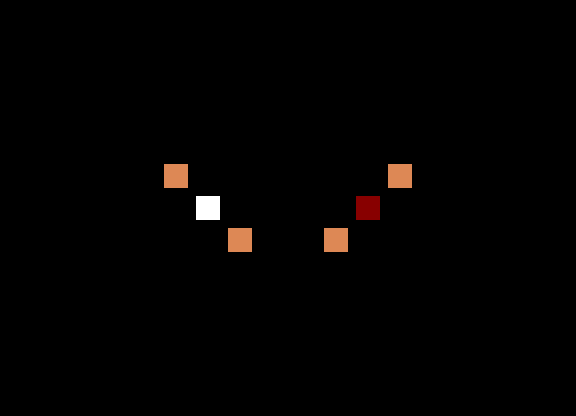
\includegraphics[width=1.3cm]{src/batalyx_patterns/pixels/pixel_pattern0_3.png}%
            
\includegraphics[width=1.3cm]{src/batalyx_patterns/pixels/pixel_pattern0_4.png}%
            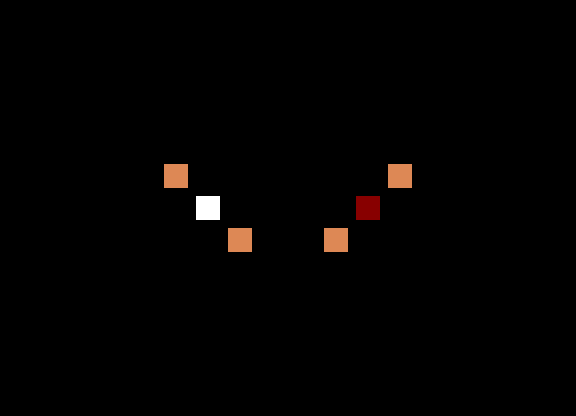
\includegraphics[width=1.3cm]{src/batalyx_patterns/pixels/pixel_pattern0_5.png}%
            } \\
            \midrule

            \makecell[l]{
              \icode{.BYTE \$FE,\$02}\\
              \icode{.BYTE \$FE,\$02}
              } & \makecell[l]{
                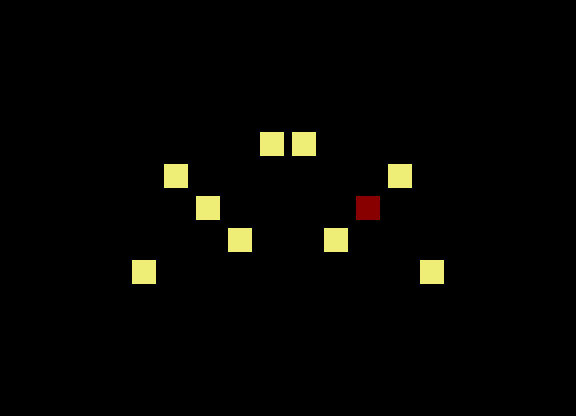
\includegraphics[width=1.3cm]{src/batalyx_patterns/pixels/pixel_pattern0_6.png}%
                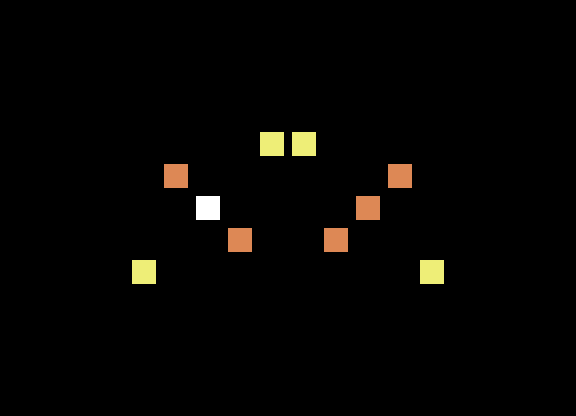
\includegraphics[width=1.3cm]{src/batalyx_patterns/pixels/pixel_pattern0_7.png}%
                
\includegraphics[width=1.3cm]{src/batalyx_patterns/pixels/pixel_pattern0_8.png}%
                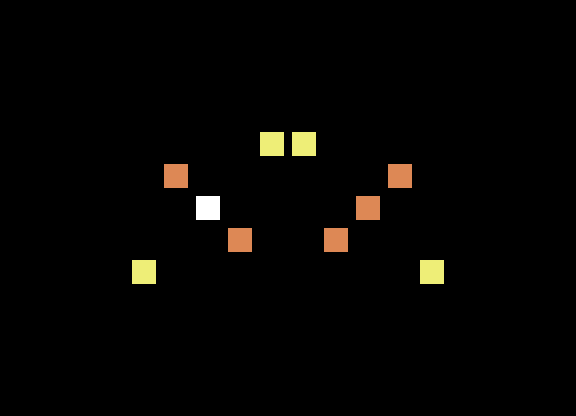
\includegraphics[width=1.3cm]{src/batalyx_patterns/pixels/pixel_pattern0_9.png}%
                } \\
                \midrule

                \makecell[l]{
                  \icode{.BYTE \$FD,\$03}\\
                  \icode{.BYTE \$03,\$FD}
                  } & \makecell[l]{
                    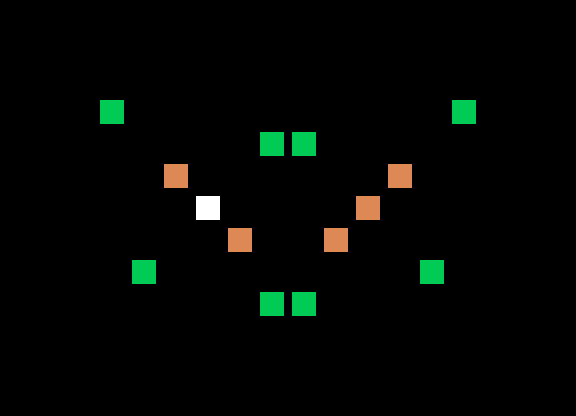
\includegraphics[width=1.3cm]{src/batalyx_patterns/pixels/pixel_pattern0_10.png}%
                    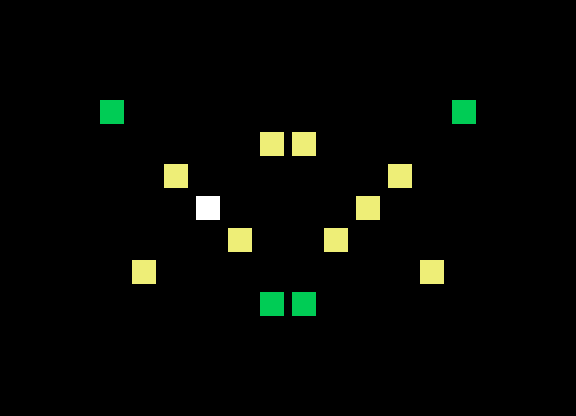
\includegraphics[width=1.3cm]{src/batalyx_patterns/pixels/pixel_pattern0_11.png}%
                    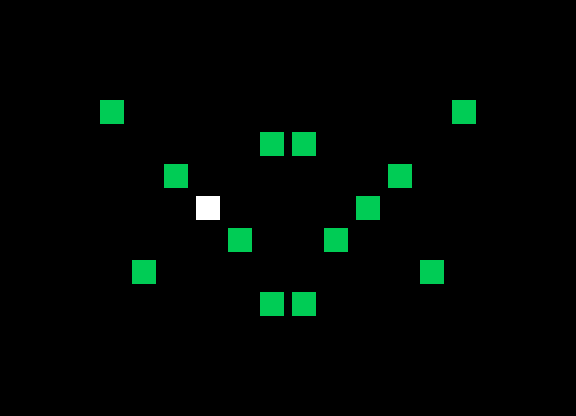
\includegraphics[width=1.3cm]{src/batalyx_patterns/pixels/pixel_pattern0_12.png}%
                    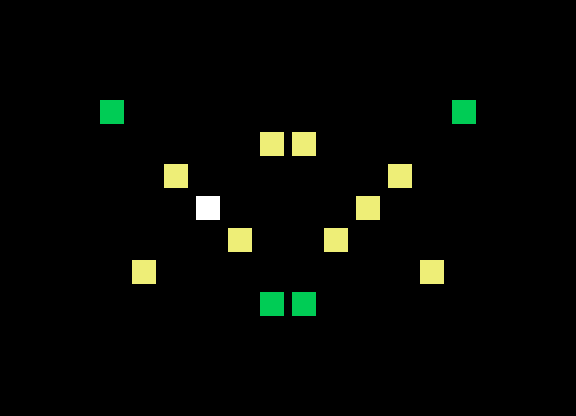
\includegraphics[width=1.3cm]{src/batalyx_patterns/pixels/pixel_pattern0_13.png}%
                    } \\
                    \midrule
      \end{tabular}
    \end{adjustbox}
  }
\end{figure}

As before, once the lines is ready to be processed the heavy lifting passes to \icode{PaintPixel\index{PaintPixel}\-ForCurrentSymmetry}.

\clearpage
\textbf{Lines 543-601. \icode{\textbf{PaintPixelForCurrentSymmetry\index{PaintPixelForCurrentSymmetry}}}} 
\begin{lstlisting}[escapechar=\%]
;--------------------------------------------------------
; PaintPixelForCurrentSymmetry%\index{PaintPixelForCurrentSymmetry}%
;--------------------------------------------------------
PaintPixelForCurrentSymmetry%\index{PaintPixelForCurrentSymmetry}%   
        LDA initialPixelYPosition
        AND #$80
        BEQ CanPaintPixelOnThisLine

CleanUpAndReturn   
        RTS 

CanPaintPixelOnThisLine   
        LDA initialPixelYPosition
        CMP #TOP_Y_POSITION+1
        BPL CleanUpAndReturn

        LDA initialPixelXPosition
        AND #$80
        BNE CleanUpAndReturn

        LDA initialPixelXPosition
        CMP #NUM_COLS
        BPL CleanUpAndReturn

        LDA currentColor
        TAX 
        LDA colorComparisonArray,X
        STA lastColorValue
        DEC lastColorValue

        JSR PaintPixel%\index{PaintPixel}%

        LDA currentSymmetrySettingForStep%\index{currentSymmetrySettingForStep}%
        BNE HasSymmetry

ReturnFromSymmetry   
        RTS 

HasSymmetry   
        CMP #X_Y_SYMMETRY
        BEQ HasXYSymmetry

        CMP #X_AXIS_SYMMETRY
        BEQ HasXAxisSymmetry

        LDA #NUM_COLS-1
        SEC 
        SBC initialPixelXPosition
        STA initialPixelXPosition

\end{lstlisting}
\clearpage
\textbf{Lines 601-625. \icode{\textbf{PaintPixelForCurrentSymmetry\index{PaintPixelForCurrentSymmetry}} continued.}} 
\begin{lstlisting}[caption = The routine responsible for handling the symmetry in use for painting pixels.,escapechar=\%]

        JSR PaintPixel%\index{PaintPixel}%

        LDA currentSymmetrySettingForStep%\index{currentSymmetrySettingForStep}%
        CMP #Y_AXIS_SYMMETRY
        BEQ ReturnFromSymmetry

        LDA #TOP_Y_POSITION
        SEC 
        SBC initialPixelYPosition
        STA initialPixelYPosition

        JSR PaintPixel%\index{PaintPixel}%

        LDA #NUM_COLS-1
        SEC 
        SBC initialPixelXPosition
        STA initialPixelXPosition

        JMP PaintPixel%\index{PaintPixel}%

HasXYSymmetry   
        LDA #TOP_Y_POSITION
        SEC 
        SBC initialPixelYPosition
        STA initialPixelYPosition

        JMP PaintPixel%\index{PaintPixel}%

HasXAxisSymmetry   
        LDA #NUM_COLS-1
        SEC 
        SBC initialPixelXPosition
        STA initialPixelXPosition
        JMP HasXYSymmetry
\end{lstlisting}

\rhead[]{\icode{PaintPixelForCurrentSymmetry\index{PaintPixelForCurrentSymmetry}}}
\textbf{Lines 543-625. \icode{\textbf{PaintPixelForCurrentSymmetry\index{PaintPixelForCurrentSymmetry}}}:} This routine feels like an improvement on
previous iterations. It makes heavy use of 'early returns' (\icode{CleanUpAndReturn}) and the way in which it is
determining what symmetry is in effect and how to decompose that into the painting of individual pixels is much more
legible to the reader than in earlier versions of the routine in Psychedelia and the 'listing edition' of Psychedelia.

\clearpage

\textbf{Lines 504-528. \icode{\textbf{PaintPixel\index{PaintPixel}}}} 
\begin{lstlisting}[caption = All the pattern data structures in Psychedelia organized into a set of arrays.,escapechar=\%]
;--------------------------------------------------------
; PaintPixel%\index{PaintPixel}%
;--------------------------------------------------------
PaintPixel%\index{PaintPixel}%   
        LDX initialPixelYPosition
        LDY initialPixelXPosition
        LDA screenLinesLoPtrArray,X
        STA colorRAMLoPtr
        LDA screenLinesHiPtrArray,X
        CLC 
        ADC #OFFSET_TO_COLOR_RAM
        STA colorRAMHiPtr
        LDA (colorRAMLoPtr),Y
        AND #$0F
        CMP currentColorValue
        BEQ ActuallyPaintPixel%\index{ActuallyPaintPixel}%

        TAX 
        LDA colorComparisonArray,X
        CMP lastColorValue
        BEQ ActuallyPaintPixel%\index{ActuallyPaintPixel}%
        BPL ActuallyPaintPixel%\index{ActuallyPaintPixel}%
        RTS 

ActuallyPaintPixel%\index{ActuallyPaintPixel}%   
        LDA currentColor
        STA (colorRAMLoPtr),Y
        RTS 

colorComparisonArray   
        .BYTE ORANGE,ORANGE,WHITE,ORANGE,BLUE,PURPLE,YELLOW,CYAN
        .BYTE RED,ORANGE,ORANGE,ORANGE,ORANGE,ORANGE,GREEN,ORANGE
        .BYTE ORANGE

\end{lstlisting}
\clearpage

\rhead[]{\icode{PaintPixel\index{PaintPixel}}}
\textbf{Lines 504-528. \icode{\textbf{PaintPixel\index{PaintPixel}}}:} This is much less cryptic than previous versions of this routine. The first part
simply figures out if the current location chosen for drawing is the same as the current background color (\icode{currentColorValue}) - if so,
we paint it.

Otherwise, we check the current color at the chosen location against the \icode{color\-ComparisonArray} using the color value itself as an index.
If it's greater or equal we paint our new chose color there.

\section*{\string^ \string^ \string^ \string^ \string^ transmission interrupted}
\vspace{-0.3cm}
OK I've had enough for now, and let's face it so have you. There's a second part to this book yet to be completed: a similar 'mirror' exploration
of Jeff Minter\index{Minter}'s second adventure in light synthesizers: 'Colourspace' for the Atari 800. The dismembered parts of this second volume are available
to preview by clicking the link below (or by visiting \href{https://github.com/mwenge/psypixels}{\textcolor{blue}{ this book's Github repository}}). 

I hope you've enjoyed this long tour through a very short computer program. Goodbye and thank you for reading!

\vspace*{\fill}
\begin{figure}[H]
    \centering
\href{https://github.com/mwenge/psypixels}{
      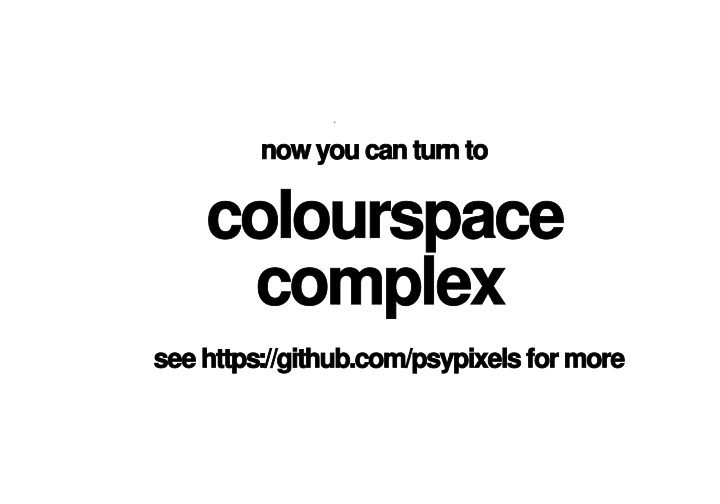
\includegraphics[width=10cm]{src/cover/title_page_colorspace_coming_soon.png}%
}
\end{figure}

\vspace*{\fill}
